% HLS4ML

\chapter{HLS4ML} % Main chapter title

\label{HLS4ML} % For referencing the chapter elsewhere, use \ref{HLS4ML} 

%----------------------------------------------------------------------------------------

\section{Description de HLS4ML}

Le paquet \acrshort{hls4ml} est un outil publié en juin 2018 par Javier Duartea et al., ayant pour but de traduire des modèles de machine learning développés en Python à l'aide de bibliothèques comme Keras ou Pytorch, en code VHDL ou Verilog pour \acrshort{fpga} \cite{duarte_fast_2018}.

Au fil du temps, ce dernier a été étendu et amélioré notamment pour son utilisation avec des réseaux neuronaux convolutifs \cite{aarrestad_fast_2021} et \cite{ghielmetti_real-time_2022}.

En plus de proposer des implémentations de faible latence, \acrshort{hls4ml} permet de développer rapidement des prototypes de modèles de machine learning sans de grandes connaissances des langages VHDL ou Verilog, tout en préservant les ressources matérielles disponibles.

\section{HLS4ML et Vitis HLS}

Comme son nom l'indique, l'outil \acrfull{hls4ml} fonctionne conjointement avec Vitis \acrfull{hls}. En effet, lors du flux de travail que nous verrons plus en détail à la section suivante (\ref{hls4ml_workflow}), le code Python est transformé en code C++ qui est converti en un projet \acrshort{hls} puis synthétisé en code VHDL ou Verilog. Bien qu'il existe différents outils pour gérer des projets \acrshort{hls}, nous nous concentrerons sur Vitis \acrshort{hls} qui est officiellement supporté par \acrshort{hls4ml} bien qu'encore au stade expérimental.

\acrfull{hls} est un processus de conception qui à partir d'un code écrit en ANSI C, ou C++ est capable de transformer celui-ci en \acrfull{rtl} (une méthode de conception de circuits logique) à l'aide d'un langage de description matérielle tel que VHDL ou Verilog. Ce dernier peut être alors synthétisé et implémenté sur \acrshort{fpga}.\\

Vitis \acrshort{hls} permet de développer des algorithmes sans avoir besoin d'écrire de code dans un langage de description matérielle, et ainsi d'accélérer la phase de conception. Par ailleurs, il fournit également des directives spéciales nommées pragmas permettant de contrôler et d'optimiser la synthèse du code. Un exemple de ces derniers pourrait être le pragma \textbf{HLS pipeline} qui va réduire la latence en parallélisant les commandes de la chaîne de traitement. Ainsi, comme illustré sur la figure \ref{fig:pipeline_pragma} dans le cas (B), les instructions sont organisées de manière à ce que différentes opérations soient réalisées en parallèle, plutôt que séquentiellement.

\begin{figure}[hbt!]
    \centering
    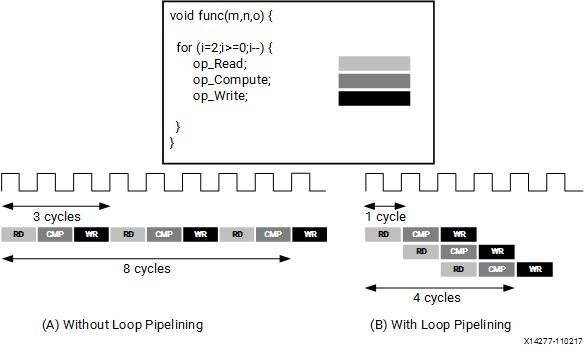
\includegraphics[scale=0.9]{Figures/hls4ml/pipeline_pragma.png}
    \caption{Exemple d'une pipeline de boucle \cite{noauthor_tme1532103642766image_nodate}.}
    \label{fig:pipeline_pragma}
\end{figure}

\break

\section{Flux de travail}
\label{hls4ml_workflow}

Le fonctionnement de \acrshort{hls4ml} peut être simplement décrit à l'aide du schéma suivant \ref{fig:hls4ml_workflow} :

\begin{figure}[hbt!]
    \centering
    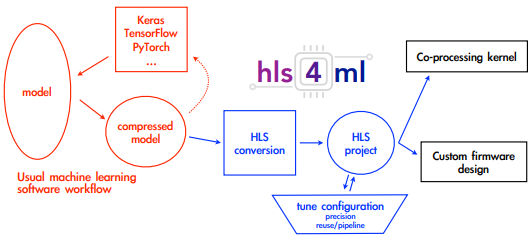
\includegraphics[scale=0.7]{Figures/hls4ml/hls4ml_workflow.png}
    \caption{Flux de travail typique lors de la conversion d'un modèle vers une implémentation \acrshort{fpga} avec \acrshort{hls4ml} \cite{duarte_fast_2018} (Figure 1)}
    \label{fig:hls4ml_workflow}
\end{figure}

Celui-ci débute par la partie illustrée en rouge, et représente les étapes habituelles de conception d'un réseau de neurones pour une tâche spécifique. Celles-ci sont réalisées avec des outils comme (Q)Keras, Tensorflow, ou Pytorch et impliquent des étapes d'entraînement, de quantification ou encore de compression avant d'obtenir le modèle final.

Le flux passe alors dans la section en bleu et converti le modèle de machine learning à l'aide de \acrshort{hls4ml} en un projet \acrshort{hls}. Celui-ci pourra être synthétisé et implémenté par la suite sur \acrshort{fpga} comme indiqué par la partie en noir.

\acrshort{hls4ml} possède un nombre de paramètres configurables afin de personnaliser au mieux la latence, l'intervalle d'initiation, ou encore les ressources utilisées par le résultat final.

\section{Fonctions (Q)Keras supportées}

Lors de la réalisation de notre travail, nous avons utilisé la version 0.7.1 de hls4ml. Bien que celle-ci propose le support de différentes bibliothèques, seule (Q)Keras est convenablement supportée, les autres étant limitées ou en cours de développement. Voici la liste des couches supportées avec la version utilisée extraite directement du code : \\

\begin{itemize}

\item\textbf{Entrée} : InputLayer.\\

\item\textbf{Convolution} : Conv1D, SeparableConv1D, Conv2D, SeparableConv2D, DepthwiseConv2D, QConv1D, QConv2D.\\

\item\textbf{Pooling} : MaxPooling1D, MaxPooling2D, AveragePooling1D, AveragePooling2D, GlobalMaxPooling1D, GlobalMaxPooling2D, GlobalAveragePooling1D, GlobalAveragePooling2D.\\

\item\textbf{Activation} : Activation, LeakyReLU, ThresholdedReLU, ELU, PReLU, Softmax, ReLU, QActivation.\\

\item\textbf{Normalisation} : BatchNormalization, QBatchNormalization.\\

\item\textbf{Dense} : Dense, QDense, BinaryDense, TernaryDense.\\

\item\textbf{Redimensionnement} : ZeroPadding1D, ZeroPadding2D, Flatten, Reshape, Permute.\\

\item\textbf{Autres} : QConv2DBatchnorm, UpSampling1D, UpSampling2D, Embedding, GarNet, GarNetStack, SimpleRNN, LSTM, GRU, Add, Subtract, Multiply, Average, Maximum, Minimum, Concatenate, Dot.\\

\end{itemize}

Dans notre cas, toutes les couches de notre modèle ResNet18+Tête sont supportées. Néanmoins, cela n'est pas le cas pour l'implémentation de YOLOv8 par KerasCV. Dans ce cas, il aurait été possible de les ajouter manuellement à l'aide de l'"extension API" \cite{noauthor_extension_nodate}. Cette dernière permet de définir la couche spécifique en la développant selon les critères de \acrshort{hls4ml} en Python et en C++.

\section{Limitations rencontrées}
\label{sec:hls4ml_limitations}

Lors du maniement de \acrshort{hls4ml} pour synthétiser notre modèle, nous nous sommes retrouvés face à différentes limitations :

La première d'entre elles concerne la "stratégie" utilisée par \acrshort{hls4ml} pour les différentes couches. Celle-ci peut être de type "Latency" ou "Resource" en fonction du nombre d'éléments contenus au sein d'une couche. Si ce nombre n'excède pas $4096$, il est possible d'adopter la stratégie "Latency" qui va favoriser la synthèse d'un code minimisant la latence, mais augmentant les ressources utilisées.
Inversement, lorsque les couches contiennent un nombre d'éléments supérieurs à $4096$, ces derniers doivent être utilisés avec la stratégie "Resource", qui se concentre sur l'optimisation des ressources au détriment de la latence, sous peine de faire planter la synthèse. Cette limitation est due à une limite de Vitis \acrshort{hls}, où le nombre d'éléments qu'il est capable de dérouler "unroll" est de $4096$ \cite{noauthor_hls4ml-tutorialpart6_cnnsipynb_nodate}.

La deuxième limitation concerne l'emploi du stride dans une couche de pooling. Le modèle ResNet18 utilise un stride de $(2,2)$ lors du max-pooling. Or la gestion de ce stride par \acrshort{hls4ml} génère à l'interne une opération de lecture et d'écriture simultanée qui n'est pas supportée et qui fait donc planter la synthèse.

La troisième limitation concerne la réutilisation d'une variable issue d'une couche "flatten" plus de trois fois. En effet, lors de ce cas, le message d'avertissement de la figure \ref{fig:warning_reuse_of_variable}, nous indique que cela n'est pas encore supporté par l'outil.

\begin{figure}[hbt!]
    \centering
    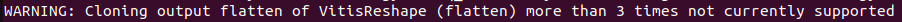
\includegraphics[scale=0.45]{Figures/hls4ml/warning_reuse_of_variable.png}
    \caption{Message d'avertissement lorsqu'une variable issue d'une couche "flatten" est réutilisée plus de $3$ fois.}
    \label{fig:warning_reuse_of_variable}
\end{figure}

La quatrième et dernière limitation rencontrée et déjà abordée dans la sous-section \ref{subsec:yolov8_utilization} concerne le déroulement des couches dans des modèles imbriqués. Cependant, il semblerait que cette limitation ait été corrigée dans une mise à jour du 16 novembre 2023 \cite{noauthor_release_nodate}.

Par ailleurs, des limitations non directement liées à \acrshort{hls4ml}, mais à la quantité de mémoire comme expliqué dans la sous-section \ref{subsec:r18_synthetize_with_hls4ml} sont également à prendre en compte.

\section{Développer et synthétiser un modèle de machine learning}

Lors de la réalisation de ce travail, nous avons commencé par prendre en main l'outil en recherchant de la documentation sur le site officiel \cite{noauthor_extension_nodate} et nous avons suivi un "tutoriel" \acrshort{hls4ml} sur comment synthétiser des réseaux neuronaux convolutifs \cite{noauthor_hls4ml-tutorialpart6_cnnsipynb_nodate}.

Bien qu'intéressants et utiles, nous avons constaté un certain manque d'informations regroupées afin de faciliter la prise en main et le développement de modèles avec l'outil. À titre d'exemple, la liste des couches supportées par \acrshort{hls4ml} a été extraite de leur code, car elle n'était pas à jour sur leur site, la limitation du nombre de réutilisations d'une variable n'a été découverte qu'au moment de la synthèse, l'utilisation d'un stride dans la couche "MaxPooling2d" déclenche une erreur même si cette dernière est censée être supportée, etc.

Ainsi, au fil du développement, nous sommes passés plusieurs fois par différentes étapes clefs pour obtenir un résultat. À partir de ces dernières, nous avons réalisé le logigramme de la figure \ref{fig:synthetize_model_with_hls4ml} présentant comment réaliser un projet de ce type à partir de zéro afin de permettre à toute personne souhaitant synthétiser son propre réseau de neurones avec \acrshort{hls4ml} de visualiser les actions à mener.\\

En parcourant celui-ci, nous commençons par développer ou tout simplement choisir le modèle désiré.

Puis, nous nous assurons que toutes les couches de ce dernier soient supportées par \acrshort{hls4ml}. Si cela n'est pas le cas, il faut vérifier si le modèle peut être adapté. Cela englobe : est-ce qu'il est possible de remplacer les couches non supportées par d'autres ? Est-ce qu'il est possible de développer soit même le code pour la couche en question ? Tout en prenant en compte les ressources nécessaires et l'impact sur le modèle de certains changements. Si cela n'est pas possible, le modèle ne peut pas être synthétisé avec \acrshort{hls4ml}. Dans le cas contraire, nous pouvons redévelopper notre modèle puis passer à la suite.

L'étape suivante n'est pas obligatoire en tant que telle pour synthétiser le modèle, mais l'inclure dans le développement permet d'obtenir un résultat plus proche de l'implémentation finale et utilisant moins de ressources.

Lorsque le réseau de neurones semble prêt à être synthétisé, nous pouvons commencer par définir la configuration de \acrshort{hls4ml}. Il faut y indiquer plusieurs informations, comme : le modèle de \acrshort{fpga} utilisé, le "reuse factor", la stratégie à adopter, la précision, etc.

Nous pouvons à présent synthétiser notre modèle. L'outil va travailler puis générer une sortie. À ce moment là nous savons si \acrshort{hls4ml} a réussi la synthèse ou non. Dans le cas où cela a été un échec, nous pouvons retrouver les erreurs rencontrées et les analyser. Nous avons retenu deux cas, les erreurs provoquées par la configuration \acrshort{hls4ml}, et celles liées au modèle. Dans le premier cas, il suffit d'adapter la configuration, et dans le second il est nécessaire de repasser par une phase d'analyse de l'erreur et d'évaluer si le modèle peut être adapté.

Finalement, si le modèle a été synthétisé avec succès, il nous est possible d'accéder au rapport de synthèse. Celui-ci nous permet d'analyser les ressources utilisées, la latence, ou encore l'\acrfull{ii}, et de modifier la configuration si le résultat n'est pas satisfaisant, par exemple : trop de ressources utilisées, une latence trop élevée, etc., jusqu'à obtenir un résultat qui nous convienne.

Une contrainte externe, déjà abordée dans la sous-section \ref{subsec:r18_synthetize_with_hls4ml}, peut venir affecter le logigramme décrit. Il s'agit de la mémoire vive utilisée. En effet, la taille du modèle et la configuration de \acrshort{hls4ml} vont venir impacter cette dernière. Il est alors nécessaire de soit modifier la configuration, soit diminuer la taille du modèle, ou le cas échéant d'utiliser une machine avec plus de ressources.\\

Comme nous venons de le voir, synthétiser un modèle avec \acrshort{hls4ml} impose des contraintes dès son développement. En prenant en compte celles-ci et les limitations de l'outil, il est alors possible d'en tirer toute la puissance.

\begin{figure}[hbt!]
    \centering
    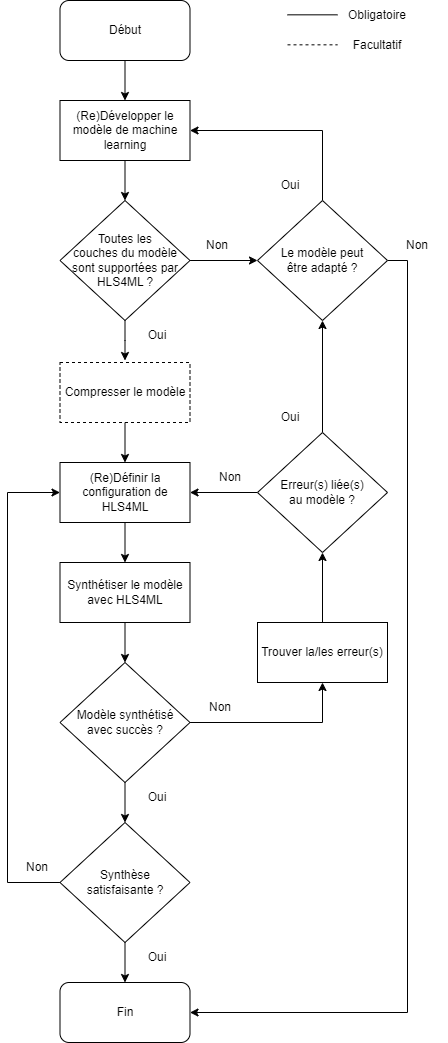
\includegraphics[scale=0.56]{Figures/hls4ml/synthetize_model_with_hls4ml.png}
    \caption{Logigramme de développement d'un modèle de machine learning et de synthèse avec \acrshort{hls4ml}.}
    \label{fig:synthetize_model_with_hls4ml}
\end{figure}

%----------------------------------------------------------------------------------------
